\input{../preamble.tex}

\SetDate[06/05/2026]

\begin{document}
\pagestyle{fancy}
\fancyhead[L]{Première spécifique}
\fancyhead[C]{\textbf{Informations chiffrées}}
\fancyhead[R]{\today}

\framebox(450,110){
	
}

\exe{}{
	Voici deux séries de valeurs.
	Série A : 1 ; 2 ; 3 et série B : 0,5 ; 2 ; 100.
	
	Quelles propositions sont vraies ?
	\begin{enumerate}[label=\textbf{\alph*.}]
		\item Les deux séries ont la même moyenne et la même médiane.
		\item Les deux séries ont la même moyenne mais pas la même médiane.
		\item Les deux séries ont la même médiane mais pas la même moyenne.
		\item Les deux séries n'ont ni la même moyenne ni la même médiane.
	\end{enumerate}
}{exe:aut0-1-12}{
	TODO
}

\exe{}{
	On considère les deux séries ci-dessous.
	Série A : 9 ; 10 ; 10 ; 11
	et
	série B : 7 ; 10 ; 10 ; 13.
	
	Quelles propositions sont vraies ?
	\begin{enumerate}[label=\textbf{\alph*.}]
		\item La moyenne de la série A est strictement supérieure à la moyenne de la série B.
		\item La moyenne de la série B est strictement supérieure à la moyenne de la série A.
		\item L'écart-type de la série A est strictement supérieur à l'écart-type de la série B.
		\item L'écart-type de la série B est strictement supérieur à l'écart-type de la série A.
	\end{enumerate}
}{exe:aut0-2-12}{
	TODO
}





\exemulticols{}{
	Une chanteuse analyse en détails ses revenus.
	Elle constate qu'un tiers proviennent des ventes de CD et vinyles, un quart des droits d'auteurs, 10\% des concerts, et le reste du streaming en ligne.
	
	Compléter le tableau ci-dessous et représenter les données avec un diagramme circulaire.
	
	
	\begin{center}
\def\arraystretch{1.5}
\setlength\tabcolsep{10pt}
		\begin{tabular}{|c|c|c|c|c|}\hline
		Catégorie & CD et vinyles & Droits d'auteur & Concerts & Streaming \\\hline
		Proportion (en \% arrondi à $10^{-1}$) & & & & \\\hline
		Angle (en °) & & & & \\\hline
		\end{tabular}
		%
	\end{center}
}{
	\begin{center}
\def\radius{2}
  \begin{tikzpicture}
        \draw (0,0)-- (0:2) arc (0:360:2);
  \end{tikzpicture}
  \end{center}
}{exe:diag-circ}{
	\begin{center}
\def\angle{150}
\def\radius{2}
\def\cyclelist{{"GREEN_E","GOLD_E","RED_E","BLUE_E"}}
\newcount\cyclecount \cyclecount=-1
\newcount\ind \ind=-1
  \begin{tikzpicture}
      \foreach \percent/\name in {
        33.3/{CD/Vinyles},
        25/{Droits d'auteur},
        10/{Concerts},
        31.7/{Streaming}
    } {
      \ifx\percent\empty\else               % If \percent is empty, do nothing
        \global\advance\cyclecount by 1     % Advance cyclecount
        \global\advance\ind by 1            % Advance list index
        \ifnum3<\cyclecount                 % If cyclecount is larger than list
          \global\cyclecount=0              %   reset cyclecount and
          \global\ind=0                     %   reset list index
        \fi
        \pgfmathparse{\cyclelist[\the\ind]} % Get color from cycle list
        \edef\color{\pgfmathresult}         %   and store as \color
        % Draw angle and set labels
        \draw[fill={\color!50},draw={\color}] (0,0) -- (\angle:\radius)
          arc (\angle:\angle+\percent*3.6:\radius) -- cycle;
        \node at (\angle+0.5*\percent*3.6:0.7*\radius) {\percent\,\%};
        \node[pin=\angle+0.5*\percent*3.6:\name]
          at (\angle+0.5*\percent*3.6:\radius) {};
        \pgfmathparse{\angle+\percent*3.6}  % Advance angle
        \xdef\angle{\pgfmathresult}         %   and store in \angle
      \fi
    };
  \end{tikzpicture}
  \end{center}
}


\exemulticols{}{
	Pour la série statistiques décrite par le diagramme à barres ci-contre, donner
		\begin{enumerate}[label=\roman*)]
			\item l'effectif total ;
			\item la moyenne ; et
			\item la médiane.
		\end{enumerate}
	Sans connaître la valeur exacte de chaque note, on assignera la valeur moyenne à chaque intervalle.
	Par exemple, du diagramme, on lit 5 notes de valeur 11,5 car situées entre 11 et 12.
	\vfill\null
}{
\begin{center}
  \begin{tikzpicture}[scale=.9]
    \begin{axis}[
        ymin=0, ymax=5,
        xmin=0, xmax=20,
        minor x tick num = 1,
        %minor y tick num=1,
        axis line style = -,
        xtick distance=2,
        area style,
        xlabel = {Note sur $20$},
        ylabel = {Effectif},
        xlabel near ticks,
        ylabel near ticks,
		extra x ticks={0},
		extra y ticks={0},
		x=10pt,
		ybar,
		bar width=8pt,
      ]
      \addplot+[bar shift=4pt,draw=BLACK, thick, fill=BLUE_E!50] plot coordinates {
        (5,1)
        (7,1)
        (9,2)
        (10,2)
        (11,5)
        (12,4)
        (13,2)
        (14,2)
        (15,4)
        (16,3)
        (17,3)
        (18,5)
        (19,1)
      };
    \end{axis} 
  \end{tikzpicture}
\end{center}

}{exe:7}{
}


\exemulticols{, difficulty=0}{
	Soient $f(x) = ax+b$ et $g(x) = a'x+b'$ deux fonctions affines données graphiquement pour $3,2 \leq x \leq 3,7$ ci-contre.
	
	\begin{enumerate}
		\item
		Pour chaque droite, donner deux points $A$ et $B$ lui appartenant.
		\item
		Déterminer les paramètres $a, b, a',$ et $b'$.
	\end{enumerate}
	
	\vfill
	
	\emph{Formules :}
	\begin{align*}
		a = \dfrac{y_B-y_A}{x_B-x_A} && \et && b =y_A - ax_A
	\end{align*}
	
	%\vfill\null
}{
	\begin{center}
	\begin{tikzpicture}[>=stealth, scale=.8]
	\begin{axis}[xmin = 3.2, xmax=3.7, ymin=5, ymax=7, axis x line=middle, axis y line=middle, axis line style=->, xtick distance=.1, ytick distance = 1,  enlargelimits=.1, grid=both, clip=true, minor x tick num = 1, minor y tick num = 3, x=500pt]
		
		% Cf
		\addplot[BLUE_E, very thick, domain =3.2:3.7, samples=2] {-1+2*x}  node[pos = .9, above left] {$\C_f$};
		\addplot[BLUE_E, very thick, dashed, domain =3.1:3.2, samples=2] {-1+2*x} ;
		\addplot[BLUE_E, very thick, dashed, domain =3.7:3.8, samples=2] {-1+2*x};
		
		% Cg
		\addplot[RED_E, very thick, domain =3.2:3.7, samples=2] {13-2*x}  node[pos = .9, below left] {$\C_g$};
		\addplot[RED_E, very thick, dashed, domain =3.1:3.2, samples=2] {13-2*x};
		\addplot[RED_E, very thick, dashed, domain =3.7:3.8, samples=2] {13-2*x};
	\end{axis}
	\end{tikzpicture}
	\end{center}
}{exe:extrapolation-graphique1}{
	Cherchons d'abord $a$ et $b$, paramètres de la fonction affine $f$.
	
	\underline{Calcul de $a$}
	
	En connaissant deux points $A$ et $B$ de $\C_f$, on peut immédiatement déduire un vecteur directeur (par exemple $\vec{AB}$) et le coefficient directeur de $f$.
	D'après le cours, ceci est équivalent à calculer 
		\[ a = \dfrac{y_B - y_A}{x_B - x_A}. \]
	Graphiquement, on lit $A(3,25 ; 5,5)$ et $B(3,5 ; 6)$, desquel on déduit
		\[ a = \frac{6-5,5}{3,5-3,25} = 2. \]
	
	\underline{Calcul de $b$}
	
	Nous ne disposons pas de point d'abscisse nulle duquel lire l'ordonnée à l'origine simplement.
	Cependant, comme $a =2$, nous savons que $f(x) = 2x+b$.
	De plus, comme $A\in\C_f$, nous pouvons obtenir la relation $y_A = f(x_A)$, qui n'admet qu'une seule inconnue, $b$, et qui permet donc de trouver la valeur de l'ordonnée à l'origine.
	\begin{align*}
		y_A = 5,5 &= f(x_A) \\
					&= f(3,25) \\
					&= 2\cdot3,25 + b \\
					&= 6,5 + b
	\end{align*}
	Il suit donc que $5,5 = 6,5+b$ et donc que $b = 5,5-6,5 = -1$.
	
	Notons, pour nous convaincre que notre choix arbitraire de point n'influe pas le résultat, que le même raisonnement avec $B\in\C_f$ donne le même résultat :
	\begin{align*}
		y_B = 6 &= f(x_B), \\
					&= f(3,5), \\
					&= 2\cdot3,5 + b, \\
					&= 7 + b.
	\end{align*}
	Par suite, $b = 6-7 = -1$.
	
	Nous concluons que $f(x) = 2x - 1$.
	
	
	En procédant similairement, nous obtenons $g(x) = -2x + 13$. (Ou $13-2x$ si on cherche à minimiser l'encre utilisée pour écrire l'expression.)
}



\exe{}{
	Une entreprise décide de mettre un nouveau produit sur le marché. Pour déterminer son prix de vente, elle réalise plusieurs tours
	de vente limités en faisant varier le prix unitaire. Les résultats obtenus sont donnés dans le tableau ci-dessous.
	
	\begin{multicols}{2}
	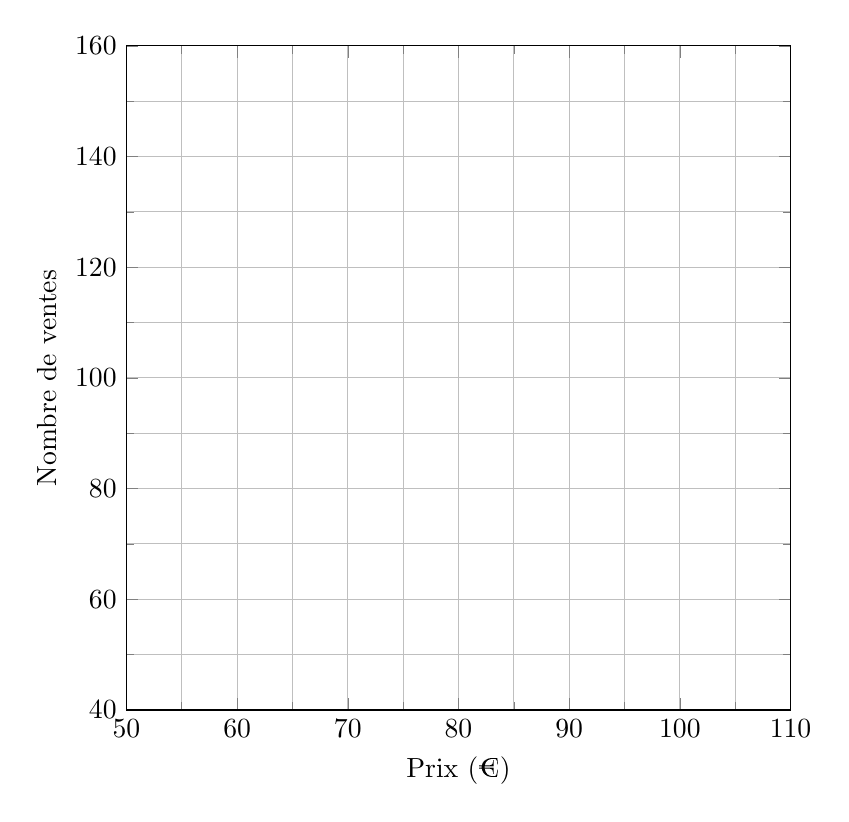
\begin{tikzpicture}
	\begin{axis}[
 		axis line style=->,
		grid=both,
		minor tick num=1,
		xtick distance=10,
		ytick distance=20,
		x=4pt,
		y=2pt,
		xmin=50,
		xmax=110,
		ymin=40,
		ymax=160,
		xlabel = Prix (€),
		ylabel = Nombre de ventes,
		ylabel near ticks,
		xlabel near ticks,
		clip=true,
		]
		%\addplot[only marks, BLUE_E, mark size=2pt]  coordinates {(50,150)(55,138)(60,130)(80,92)(100,48)}; 
	\end{axis}
	\end{tikzpicture}
\def\arraystretch{2}
\setlength\tabcolsep{10pt}
	\null\hfill
	\begin{tabular}{|c|c|c|}
		\hline
		\textbf{Prix} & \textbf{Ventes} & \textbf{Recettes}
		\\\hline
		50 & 150 & \\ \hline
		55 & 138 & \\ \hline
		60 & 130 & \\\hline
		65 &  & \\\hline
		70 &  & \\\hline
		75 &  & \\\hline
		80 & 92 & \\ \hline
		90 &  & \\\hline
		100 & 48 & \\\hline
	\end{tabular}
	\vfill\null
	\end{multicols}
	
	\begin{enumerate}
		\item
		Représenter les données du tableau dans le repère ci-dessus.
		Tracer une droite d'ajustement passant approximativement par les points.
		\item 
		Déterminer l'équation de la droite tracée liant le nombre de ventes $y$ et le prix $x$ sous la forme $y=ax+b$.
		Arrondir les paramètres $a$ et $b$ à l'unité.
		\item 
		À l'aide de cette droite, remplir la colonne « Ventes » du tableau.
		\item 
		Selon vous, quel est le prix permettant à l'entreprise de réaliser le plus grand chiffre d'affaire ?
		Remplir la colonne « Recettes » du tableau pour répondre à la question.
	\end{enumerate}
 
}{exe:recettes}{
	\begin{center}
	\begin{tikzpicture}
	\begin{axis}[
 		axis line style=->,
		grid=both,
		minor tick num=1,
		xtick distance=10,
		ytick distance=20,
		x=4pt,
		y=2pt,
		xmin=50,
		xmax=110,
		ymin=40,
		ymax=160,
		xlabel = Prix (€),
		ylabel = Nombre de ventes,
		ylabel near ticks,
		xlabel near ticks,
		clip=true,
		]
		\addplot[only marks, BLUE_E, mark size=2pt]  coordinates {(50,150)(55,138)(60,130)(80,92)(100,48)}; 
	\end{axis}
	\end{tikzpicture}
	\end{center}
}



%%%%%%%%%%%%

\newpage
\fancyhead[C]{\textbf{Solutions}}
\shipoutAnswer

\end{document}
